\documentclass[titlepage]{article}
\usepackage[a4paper, total={6in, 9in}]{geometry}
\setlength{\tabcolsep}{11pt}
\usepackage{float}
\usepackage{graphicx}

\begin{document}

\title{
  CS455: Term Project Report\\
  \large Analyzing Residential Zoning in the United States\\
}

\author{Ayush Adhikari, Brendan Verspohl}

\maketitle

\section{Introduction}
Zoning has been used for many decades in the United States to separate industrial, commercial, and residential sectors, but it was also once a motivation to segregate people of different races and classes. Governments designated some areas for residential use, which were predominantly used to build spacious single-family homes that appealed to middle-class families. This suburban development, which often prohibited multi-family homes and imposed a minimum lot size, was appealing to white families wanting to escape the urban environment that was increasing in racial diversity and limited housing options. Families with lower income could not afford to live in these areas and were pushed towards red-lined areas. Through the expansion of highways, suburbs became more accessible and popular, but it also hindered progress towards inclusive communities as suburbs became isolated and reliant on cars rather than public transport \cite{freemark}. Most developed European and Asian cities have a longer history than the United States and employ a more inclusive zoning where buildings are not strictly used for one purpose \cite{hertz}. This allows residents to be closer to commerce and one another, often reducing the need for cars and long commute times, and therefore, the carbon footprint \cite{romem}. 

With an effective zoning policy, governments can incentivize subsidized housing, public transportation, better land use, and policies that discourage displacement of people with low incomes. With this project, we look to compare the effects on quality of life and standard of living as a result of single-family housing in different areas of the United States, and possibly the world. We considered aspects such as unemployment, commute, poverty, mental health, occupancy, lot sizes, rent, etc. \cite{kaggle}. While some of these are harder to measure and compare, others provided a good insight into our hypothesis that single family residential zoning results in a worse standard of living \cite{uscensus}. For the analysis, we employed Spark with Java and Gradle and Python for the final presentation and discussion of our results. 

This paper is structured  as follows. Section 2 defines the technical description of the problem and section 3 identifies approaches and implementations with their advantages and disadvantages of that problem. We detail more on our implementation and the tools we used in section 4 and lead on to section 5 with results on the benchmarks and analysis. Sections 6 and 7 are reflections on the project and detail how the project could be improved and what we learned. Finally, section 7 concludes the paper.


\section{Problem Characterization}
Our exploration began with a fundamental question: How does the type of zoning such as: single-family or multi-family, affect the community? It's a question that demands a deep dive into the intricate relationship between zoning policies and community well-being. To tackle this question effectively, we recognized the need to approach it from various angles. This caused us to not be able to simply rely on data as we needed to look at the historical context allowing us to uncover the underlying narratives and understand the lived experiences of residents in these zoning types. 

Delving into the historical context of zoning regulations was a necessity. By understanding the origins and evolution of these policies, it allowed us to grasp their long-term impacts on neighborhood dynamics as well as societal equity. This also gave us some key insights like how historically, American zoning laws primarily revolved around the single-family home. One such historical narrative is that this was driven by the necessity to safeguard property values threatened by emerging forms of transportation. \cite{History}.

However, history alone could not provide us with the holistic view in which we needed. Thus, to complement our historical knowledge of the subject we needed to perform an analysis with concrete data on key indicators of quality of life such as: employment rates, commute times, housing affordability, commute time, car ownership, and many more. By collecting and analyzing this data with multiple different methods, we aimed to uncover patterns and correlations that could shed light on the impact of zoning on community well-being, quality of life and other indicators. 

We also wanted to push forward and expand outwards to look at the global perspective. Mainly we wanted to target more such as: European and Asian zoning. Zoning in these countries are typically not structured in the way that American zoning is. This would allow us to have a more diverse and holistic view of how these zoning practices affect the wellbeing of a community based on their cultural background. We would have liked to perform a direct data analysis between all of these countries' data but that would prove to be difficult due to the laws that prevent that data from being accessed outside of the US.

\section{Dominant Approaches}
Our journey into understanding the impacts of zoning regulations on communities led us to use two primary approaches. These are needing a historical understanding and the other being doing data analytics on zoning data. Each approach offers unique perspectives that we can use to understand how zoning policies and quality of life indicators interact.

We first used the historical context approach as a way to understand the thought behind the zoning and the timeline of how we reached our current zoning laws. By delving into the evolution of zoning regulations, we uncovered insights into the genesis and progression of current zoning practices \cite{freemark}. This retrospective exploration helped us understand the historical reasons behind zoning decisions, revealing how societal norms and economic factors have shaped community development. This helped us immensely understand the scope of the project. However, while offering valuable context, it is constrained by what was written and documented in the time. Thus we must look at the present which will allow us to see a much more clear picture of what are the results of the historical zoning laws. 

Our second approach, data analytics provided us with an overall holistic view of what was currently happening in today’s society. This allowed us to look at zoning's impact on quality of life indicators as mentioned in the problem characterization. We thus utilized different data sources: \cite{kaggle}, \cite{isqols}, \cite{koordinates} and \cite{uscensus}. Which allowed us to correlate the different types of data with each other such as the following. We must look at how the quality of life indicators are correlated with our zoning metrics: single family housing and multi family housing. This methodology would allow us to gain insights and identify opportunities for policy intervention since we are using real world data. Thanks to another paper \cite{zoning} we were able to gain an even granular view of the zoning effects on poverty since they used quality of life indicators at an even more micro level. Our data analytics however, encountered some issues which were due to data accessibility constraints as well as most of the data was separated so we needed to preprocess it.

By using both historical context and data analytics, we are able to have a very holistic view of how  zoning affects the community. The combination of both historical narratives and an understanding of how the real world zoning and quality of life data is currently shaped we can definitely draw conclusions about what the nature of single family vs multifamily zoning does to a community.

\section{Methodology}
The planning for this project consisted of four phases that helped organize and streamline the research and development needed. These were researching, gathering data, preprocessing the data, and then a final analysis using the tools we defined. After the initial proposal, we first set out to research zoning types, residential zoning, and differences between the United States and other countries that have multi-purpose zoning laws. We narrowed down the countries to compare based on the accessibility of public datasets on zoning and standard of living. Besides the United States, these included English speaking countries such as England, Canada, Australia, etc. for the ease of translation, though we also considered other European nations as they also utilized mixed zoning development. With these considerations, we began to collect the necessary data.

The datasets needed to have some information about zoning, which we found was more common with cadastral datasets used for the purposes of taxing and recording land ownerships. As this is private information, their publicity depends on the laws of that country, which prevented us from accessing this for a lot of the countries we planned to compare to. In fact, we could not find any data on European or Asian countries that we thought would have comprehensible datasets. Even if they existed, gathering the data needed for quality of life would be another issue, which might not be compatible with the information for the US, so we planned to only focus on places within the United States. However, although the United States had county level datasets, they were not available as a collection. This meant that we could not use an API to download this data, and it forced us to navigate county websites, scavenging for any cadastral or parcel-based datasets. We were able to accumulate approximately 3 GB of data that spanned ~95 counties in the US, with most of them being in Ohio. This was because Ohio had the largest cadastral dataset available with the zoning information we required \cite{koordinates}. Others were selected from different regions of the US for a wider range of selection and distribution. These included Denver, Jefferson, and Weld County from Colorado, Dallas County and Houston from Texas, Placer County from California, and the city of Detroit, Michigan. In addition to zoning data, we also needed data to measure quality of living. We considered aspects such as unemployment, commute, poverty, mental health, occupancy, lot sizes, rent, etc. Some were easy to access using the US census, but others such as lot sizes and rent were more difficult to measure due to the differences in houses, condos, and apartments \cite{uscensus}. Our final data directory consisted of the parcel data of each place as well as files for quality of life, totaling 3.2 GB of data.

As all the data was collected separately for different use cases, it required preprocessing before the analysis. We decided to employ Apache Spark using Java and Gradle for both processes and the data itself was stored using HDFS. The diagram below details this setup. There are 6 Java files, and each consists of multiple spark jobs for preprocessing, calculating the zoning percentages, filtering out residential zoning, and processing quality of life data from the individual census datasets. The files are for the places described above categorized by their state or their name if they are singular in their state. This facilitated two types of logic in our code, one for working with JavaPairRDDs and another for JavaRDDs, but the structure for both is similar. As an example, Colorado.java reads three parcel files from HDFS for each of its counties. Each county name is set as the key and the extracted zoning information as the value. This allows us to use union to create a single RDD that encompasses all counties in Colorado. With this RDD, we can group by key and work with an iterable of zoning types. For example, we can use flatMapValues() to filter out all the values that are not residential using regex and count of all residential or just single-family lots for each county. Each job outputs its results locally to a directory called outputs that is organized by each program name. The various other jobs correspond to calculating commute time, transportation types, poverty rates, housing occupancy, and other quality of life variables. They all follow a similar logic to one another and use RDDs to extract data from the corresponding datasets, match the data to the county, calculate percentages, and save that to the output directory. The main method coordinates all of these using a single spark context. The rest of the java files are structured in a similar way but there are changes based on how the zoning is defined, where it is located, and the type of RDD and thus the methods required. They also did not require a union of datasets as they were already completed. With this, we were able to use Spark to analyze the data and extract key information, reducing the size to less than 10 MB. The next step was to analyze the data, which we did using Python. We created a numpy ndarray based on all the outputs and used that for various analysis available to view in the notebook. This consisted of extracting features relating to quality of life and correlating them against the percentage of single-family zoning for every county. We chose to graph a linear function as well as a polynomial function to fit the data.

\begin{figure}[h]
  \centering
  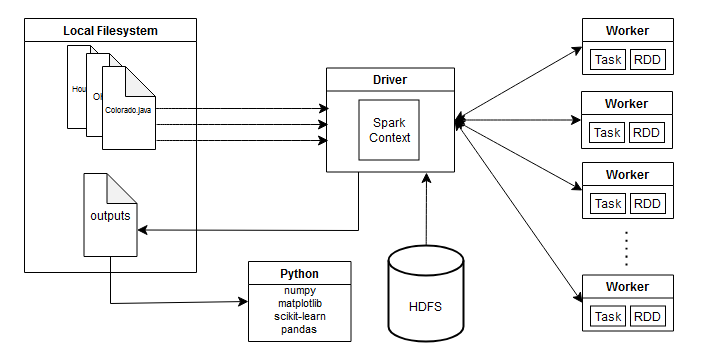
\includegraphics[width=\linewidth]{uml}
\end{figure}

\section{Experimental Benchmarks}
Due to issues with the setup, we were not able to run our clusters with the master node and instead opted to run it locally, in standalone mode using "local" and "local[*]". The difference is that the first uses only one thread while the latter utilizes all available threads on the machine. This still allowed us to benchmark the performance and throughput in terms of threads and size of the datasets. These results are shown in the table below and were measured with everything constant. Both setups were run on the same day, time, and local machine consecutively. We chose not to run them in coordination as they could have affected the results due to resource availability. Instead, we alternated which setup ran first and computed the averages of the results. The most noticeable results are in the Colorado row. In our benchmarks, this program took the longest to run despite it being a lot smaller than other datasets, which we assume is due to the union of three datasets. As mentioned above, this was the only program that utilized  unions, but everything else was similar. Besides this, there is a trend of the increase in time as the size of the dataset increases, which is expected as it requires more time to parse through a larger dataset. What is interesting is that for almost all programs, the setup using only one thread matched the performance of the other; they were all within 1-2 seconds of each other. We expected to observe the opposite effect, but we speculate this is due to the size of the datasets. The overhead of starting and stopping the threads and distributing the work detracted from the performance. If the data was larger, we think local[*] would have more impact, but it was not required for this use case.

\begin{table}[H]
  \centering
  \begin{tabular}{ |p{2cm}|p{2cm}|p{2cm}| p{2cm}| }
  \hline
    Dataset &Size &local &local[*]\\
    \hline
      Colorado & 257.5 MB &2m 42s &1m 14s \\
      Dallas & 383.3 MB &13s &14s \\
      Detroit &129.9 MB &9s &8s \\
      Houston &721.9 MB &22s &20s \\
      Ohio &1.5 GB &23s &22s \\
      Placer &187.4 MB &9s &10s \\
    \hline
  \end{tabular}
  \end{table}

In our analysis of the data with Python, we graphed the disparity between single-family and multi-family zoning. It exhibits a large gap between the two as most of the places we examined had 90\% or above of its zoning allocated for single-family. In fact, looking at the means, single-family is ~89\% and multi-residential is ~10\%. We then used the percentage of single-family zoning in the county to correlate with each of the quality of life. Of those, the most significant were related to commute. Car usage seems to be positively correlated while the usage of public transport and walking seems to be negative. This aligns with one of our hypotheses that zoning affects commute types and times. Lastly, we examined the correlation of races since our introduction to this problem stemmed from the concept of redlining. The last four graphs show that for white households, there is a positive correlation while there is a negative one for the minority races.

\section{Insights Gleaned}
Looking back on our project, we learned some important things that help us understand what went well and where we can improve. Spark Performance and Setup: We found that while we used Apache Spark that's supposed to dispatch the work across the cluster of computers, it was not using the cluster like we thought it was, thus all the computing was done on the master node. This made us dig deeper into how Spark was set up and why it wasn't using all the available resources like we thought it would allow us to. Which allowed us to improve our performance by a bit with the following. Local vs. Local[*]: We also compared two ways of running Spark, called "local" and "local[*]". Since we were not able to use the distributed nodes to compute the data we instead due to time constraints used local[*] which would allow for the computation to happen across multiple threads on the master node. Areas to Improve: Looking back, we see some things we could have done better. For example, getting good data about rent prices was tough since that data is so hard to get since many complexes have multiple different units as well as multiple different systems storing this data. Comparing Housing Metrics: We realized comparing different types of housing, like apartments and single-family homes, wasn't easy. Each type is so different, and there's no standard way to measure them. Like how we mentioned above this would be a project on its own to collect that type of data from apartments. Complexities in Lot Size Comparisons: We also saw how tricky it is to compare the sizes of lots of land. Zoning rules can change how land is used, making it hard to measure lot sizes in a meaningful way. We would have needed a deeper understanding of zoning laws in order to do a proper analysis of this data. Looking ahead, these insights will help us refine our methods, use data more efficiently, and understand that the insights that we can get would benefit from talking to a matter expert. Understanding these insights will make our future projects stronger and more effective.

\section{Future}
Start section here

\section{Conclusions}
Start section here

\bibliographystyle{unsrt}
\bibliography{references}

\end{document}
\endinput
